\title{INTD262: Number Systems in pre-Columbian Mayan Culture}
\author{Dr. Jordan Hanson - Whittier College Dept. of Physics and Astronomy}
\date{\today}
\documentclass[12pt]{article}
\usepackage[margin=1.5cm]{geometry}
\usepackage{hyperref}
\usepackage{graphicx}
\usepackage{amsmath}
\begin{document}
\maketitle

\section{Introduction}

In this activity, we will learn that written numbers are actually symbols within a larger system, and that other systems exist.  We will learn that the symbols correspond to abstract ideas that appear to be universal to human beings.  We will introduce the concepts of \textit{digits} and \textit{weights}, and four systems that use them to form numbers.  First, we will understand the binary system, arguably the simplest number system.  Second, we will understand the base-10 or Hindu-Arabic system.  Third, we will understand the base-16 or hexadecimal system.  Fourth, we will explore the base-20 or vigesimal system.  Finally, we will apply our knowledge of the vigesimal system to perform calculations as the Mayans did.

\section{Digits and Bases}

Consider the number 255.  You may have learned how to break this type of number into \textit{digits} and \textit{weights}.  There are three digits: one ``2,'' and two instances of ``5.''  What do the digits mean, given that they are not in the same location?  We know the answer from basic math courses:
\begin{equation}
255 = 2\times 100 + 5\times 10 + 5\times 1 = 2\times 10^2 + 5\times 10^1 + 5\times 10^0
\end{equation}
The left/right position of the digits determines how much \textit{weight} we give each digit.  For example, the 2 has a \textit{weight} of 100, or $10^2$.  The first 5 has a \textit{weight} of 10, or $10^1$.  The final five has a \textit{weight} of 1, or $10^0$.  The fact that the weights use powers of 10 reveals that we are using a \textit{base-10} number system.  Switching the base of our number system requires us to think on a level that resembles switching our \textit{language} that we use to speak.  Though we may grasp an idea in our mind, communicating it becomes challenging because we've changed the underlying set of symbols used to communicate.  Consider the following examples, as we switch to base-2 (\textit{binary}).

\section{Base-2 or Binary}

\begin{itemize}
\item Consider the numbers 255 and 256.  Can you identify the power of 2 that corresponds to 256?  Powers of two grow like this: 1, 2, 4, 8, 16, 32, ... ($2^0$, $2^1$, $2^2$, $2^3$, $2^4$, $2^5$). \\ \vspace{1cm}
\item Try obtaining the power of 2: (a) 512 (b) 1024 (c) 2048. \\ \vspace{1cm} 
\item Binary works with just two digits: 0 and 1.  The number of digits is the same as the base.  For the number nine, all we have to do is put a 1 in the 8's place, and add 1: $1001 = 1000 + 1$.  Convert the following \textit{decimal} numbers into binary: (a) 5 (b) 17 (c) 33. \\ \vspace{1.5cm}
\item Now write 256 in binary.  Recall that $2^8 = 256$. \\ \vspace{1cm}
\item How do you suppose we write 255 in binary?  Recall that $2^8 = 256$. Consider what you do when you write 19, as opposed to 20.  We reduce the most significant digit by one count, and change the next most significant digit accordingly. \\ \vspace{1.5cm}
\end{itemize}

\section{Base-10 or Hindu-Arabic}

\section{Base-20 or Vigesimal}

\begin{figure}[hb]
\centering
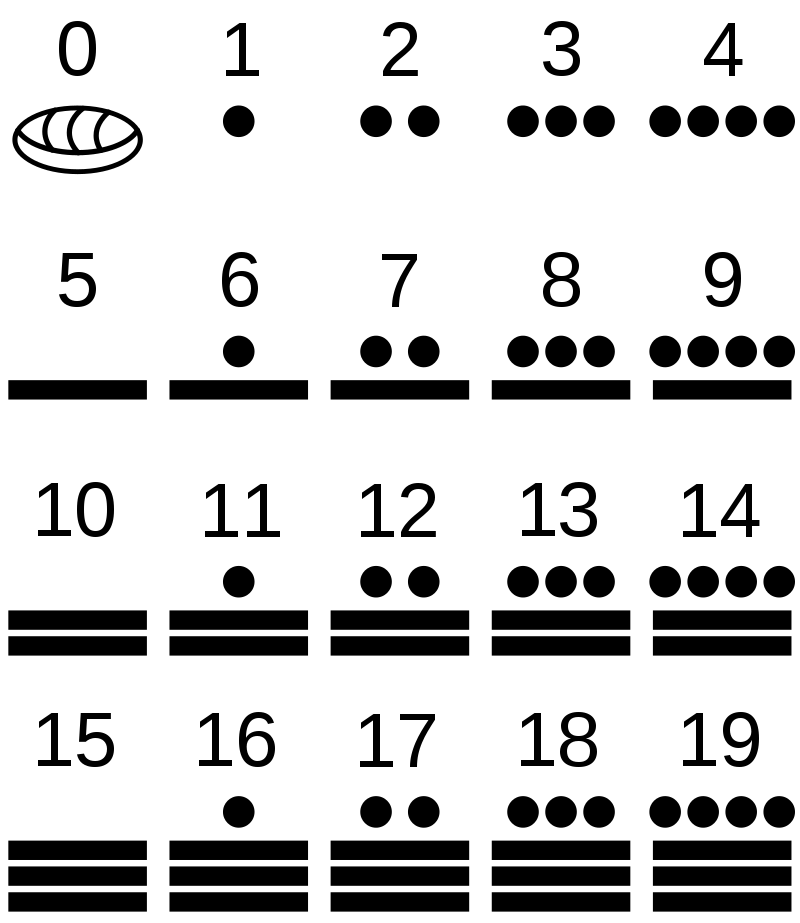
\includegraphics[width=5cm]{figures/maya_digits.png}
\caption{\label{fig:maya} The 20 digits of the Mayan system.  The digit for 0 resembles an empty shell.  The dots are worth 1 and the bars are worth 5.  In a number larger than 19, the symbols stack vertically.}
\end{figure}

\end{document}
